\documentclass[10pt,a4paper,twoside]{article}
\usepackage[a4paper,top=20mm,bottom=20mm,outer=5cm]{geometry}
\usepackage[utf8]{inputenc}
\usepackage[english]{babel}
\usepackage{graphicx}
\usepackage{hyperref}
\usepackage{cleveref}
\usepackage{natbib}
\bibliographystyle{abbrvnat}
\setcitestyle{authoryear}

\title{Project Machine Learning\\--- Milestone 1 ---}

%%%%%%%%%%%%%%%%%%%%%%%%%%%%%%%%%%%%%%%
%                                     %
%   EVERYTHING BELOW CAN BE CHANGED   %
%                                     %
%%%%%%%%%%%%%%%%%%%%%%%%%%%%%%%%%%%%%%%
\author{Max Mustermann}  % TODO: all group members
\date{\today}

\usepackage{xcolor}
% Links as dark blue text instead of hyperref's default coloured boxes.
\hypersetup{colorlinks, allcolors=blue!50!black}
\usepackage{booktabs}    % \toprule, \midrule, \bottomrule in tables
\usepackage{subcaption}  % subfigures (a), (b) side by side
\graphicspath{{figures/}}

% Shared names and notation, so every section writes them the same way.
% Use them as \tabicl{} or \nanotabicl{} (the {} keeps the space after them).

\newcommand{\tabicl}{TabICLv2}
\newcommand{\nanotabicl}{nanoTabICL}
\newcommand{\tabpfn}{TabPFNv2}
\newcommand{\tabpfnval}{\texttt{tabpfn\_val}}

% Mark open points while writing; they show up red in the PDF.
% Remove all of them before handing in (search for "\todo").
\newcommand{\todo}[1]{\textcolor{red}{[TODO: #1]}}


\begin{document}
\maketitle

% One file per section, in sections/, following the task sheet's report part.
% At most 10 pages, no code.
% !TEX root = ../report_template.tex
\section{Introduction}\label{sec:introduction}
% Not graded on its own; keep it to one short paragraph.
% - The task: given a labeled training table and unlabeled test rows, predict
%   the test labels in one forward pass (in-context learning).
% - The paper \citep{qu2026tabiclv2} and our starting point \citep{nanotabicl}.
% - What this report covers: \Cref{sec:data}, \Cref{sec:evaluation}, \Cref{sec:discussion}.

\todo{goal of the milestone, one paragraph}

% !TEX root = ../report_template.tex
\section{Dataset overview}\label{sec:data}
% 4 points. The task sheet's points are guidelines, not a checklist.

\subsection{Exploration of synthetic and real tables}\label{sec:exploration}
% What kinds of tables does the prior generate (sizes, feature types, number
% of classes, targets)? What do the benchmark datasets (\tabpfnval{},
% \citealt{hollmann2025tabpfn}) look like? Show examples made with show().

\todo{prior tables and benchmark tables, with show() figures}

\subsection{Data quality and splits}\label{sec:quality}
% Problems that could distort the evaluation: degenerate synthetic tables,
% duplicates between train and test rows, class imbalance, outliers.

\todo{what we checked and found}

\subsection{Preprocessing and representation}\label{sec:preprocessing}
% Normalization, categorical features, missing values: what and why.
% Which transformation we pass to load_data.
% Can the model handle tables of different size or shape?

\todo{preprocessing and why}

\subsection{Synthetic vs.\ real data and open questions}\label{sec:questions}
% How similar are the synthetic tables to real ones?
% What could a machine learning model answer about the data,
% and what would a human typically ask?

\todo{synthetic vs.\ real; questions a model vs.\ a human would ask}
   % 4 points
% !TEX root = ../report_template.tex
\section{Baseline and evaluation}\label{sec:evaluation}
% 3 points.

\subsection{Baseline models}\label{sec:baselines}
% Simple baselines fitted per table (k-NN, linear models, random forests,
% gradient-boosted trees) and the first approach from our prototype.
% Why these? Introduce the prototype briefly here; the paper's method is
% explained in \Cref{sec:method}.

\todo{baselines and the prototype, and why}

\subsection{Evaluation metrics and protocol}\label{sec:metrics}
% Which metrics are meaningful, and why?
% Protocol: splits, rows per dataset, which datasets are skipped.
% How do we aggregate over many datasets of different difficulty?

\todo{metrics, protocol and aggregation}

\subsection{Experimental results}\label{sec:results}
% Training and validation loss curves of the prototype; baselines vs.
% prototype on synthetic and real tables, broken down by relevant
% categories (e.g. number of classes, rows, features).
% Captions only describe; the interpretation goes in the text.

\begin{figure}
  \centering
  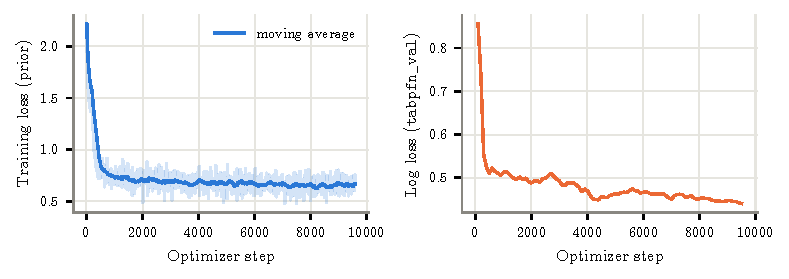
\includegraphics[width=\linewidth]{training_curves}
  \caption{Training loss on the prior (left) and log loss on the \tabpfnval{}
    datasets (right) over the optimizer steps of the 2-hour run.}
  \label{fig:training_curves}
\end{figure}

\Cref{fig:training_curves} shows \todo{what can be seen, and does it make sense?}

% Table pattern (booktabs, best value in bold):
% \begin{table}
%   \centering
%   \begin{tabular}{lrrr}
%     \toprule
%     Method & Log loss & Accuracy & ROC AUC \\
%     \midrule
%     Prototype (ours) & \textbf{0.44} & 0.84 & 0.89 \\
%     Random forest    & 0.50 & 0.82 & 0.87 \\
%     \bottomrule
%   \end{tabular}
%   \caption{Mean scores on the \tabpfnval{} datasets. Best value in bold.}
%   \label{tab:baselines}
% \end{table}

\subsection{Overfitting and failure analysis}\label{sec:overfitting}
% Is overfitting an issue? How do we check for it, and how do we avoid it?
% Where do the baselines and the prototype fail?

\todo{overfitting; where the methods fail}

\subsection{Non-technical view}\label{sec:nontechnical}
% What makes the task easy or hard, in plain words?

\todo{what makes the task easy or hard}
 % 3 points
% !TEX root = ../report_template.tex
\section{Discussion}\label{sec:discussion}
% 2 points.

\subsection{\tabicl{} method overview}\label{sec:method}
% The method of the paper \citep{qu2026tabiclv2}, briefly: what does the model
% approximate (posterior predictive, \citealt{muller2022pfn}), and how do the
% architecture and the prior achieve it?

\todo{what the model approximates; architecture and prior}

\subsection{Challenges and limitations}\label{sec:challenges}
% Why is the task not trivial?
% Why would a model trained only on synthetic data be interesting?
% Limitations of our prototype (model size, compute, datasets).

\todo{why it is hard; why synthetic-only training is interesting; limitations}

\subsection{Summary and future work}\label{sec:summary}
% What does (not) work, and why (not)?
% What is possible with our compute budget? What would we try next?

\todo{what works and what does not; next steps}
         % 2 points

% Lists every entry of the .bib, cited or not. Remove once the text cites them.
\nocite{*}
\bibliography{report_template}
\end{document}
